\begin{frame}{Challenge 1 - Signal to background separation}
\begin{block}{Problem 1}
    \begin{itemize}
        \item Separation of signal to background
        \item Signal: \tW
        \item Background: \ttbar
    \end{itemize}
\end{block}
\begin{block}{Classic approach}
    \begin{itemize}
    \item Applying a cut selection
    \end{itemize}
\end{block}
\begin{block}{Alternative}
    \begin{itemize}
        \item Machine Learning
        \item In particular: Classifying neural network
    \end{itemize}
\end{block}
\end{frame}

\begin{frame}[c]
\begin{center}
\Huge Artificial neural network
\end{center}
\end{frame}

\begin{frame}{Neural Networks - Processing information}
\begin{tabular}{p{5cm}|p{5cm}}
    \begin{figure}
    	
\includegraphics[scale = 0.09]{brain}
    \end{figure}
    & 
    \begin{figure}
    	
\includegraphics[scale = 1.4]{machine}
    \end{figure} \\
  \multicolumn{1}{c|}{Humam senses} & \multicolumn{1}{c}{Input variables} \\
    \begin{itemize}
        \item Extraction of relevant info
        \item Impossible for machines
    \end{itemize}
    & 
    \begin{itemize}
      \item Preprocessed by user
      \item {e.g.} kinematic variables
    \end{itemize} \\
\multicolumn{1}{c|}{Human brain} & \multicolumn{1}{c}{Net of nodes} \\
    \begin{itemize}
        \item Web of neuron cells
        \item Input from surrounding cells
        \item Single combination $\rightarrow$ action
    \end{itemize}
    & 
    \begin{itemize}
      \item Nodes = simple processors
      \item Connected by linear function
      \item Combination forms non-linear model
    \end{itemize} 
 \end{tabular}
\end{frame}


\begin{frame}{Neural network structure}
\begin{figure}
\centering
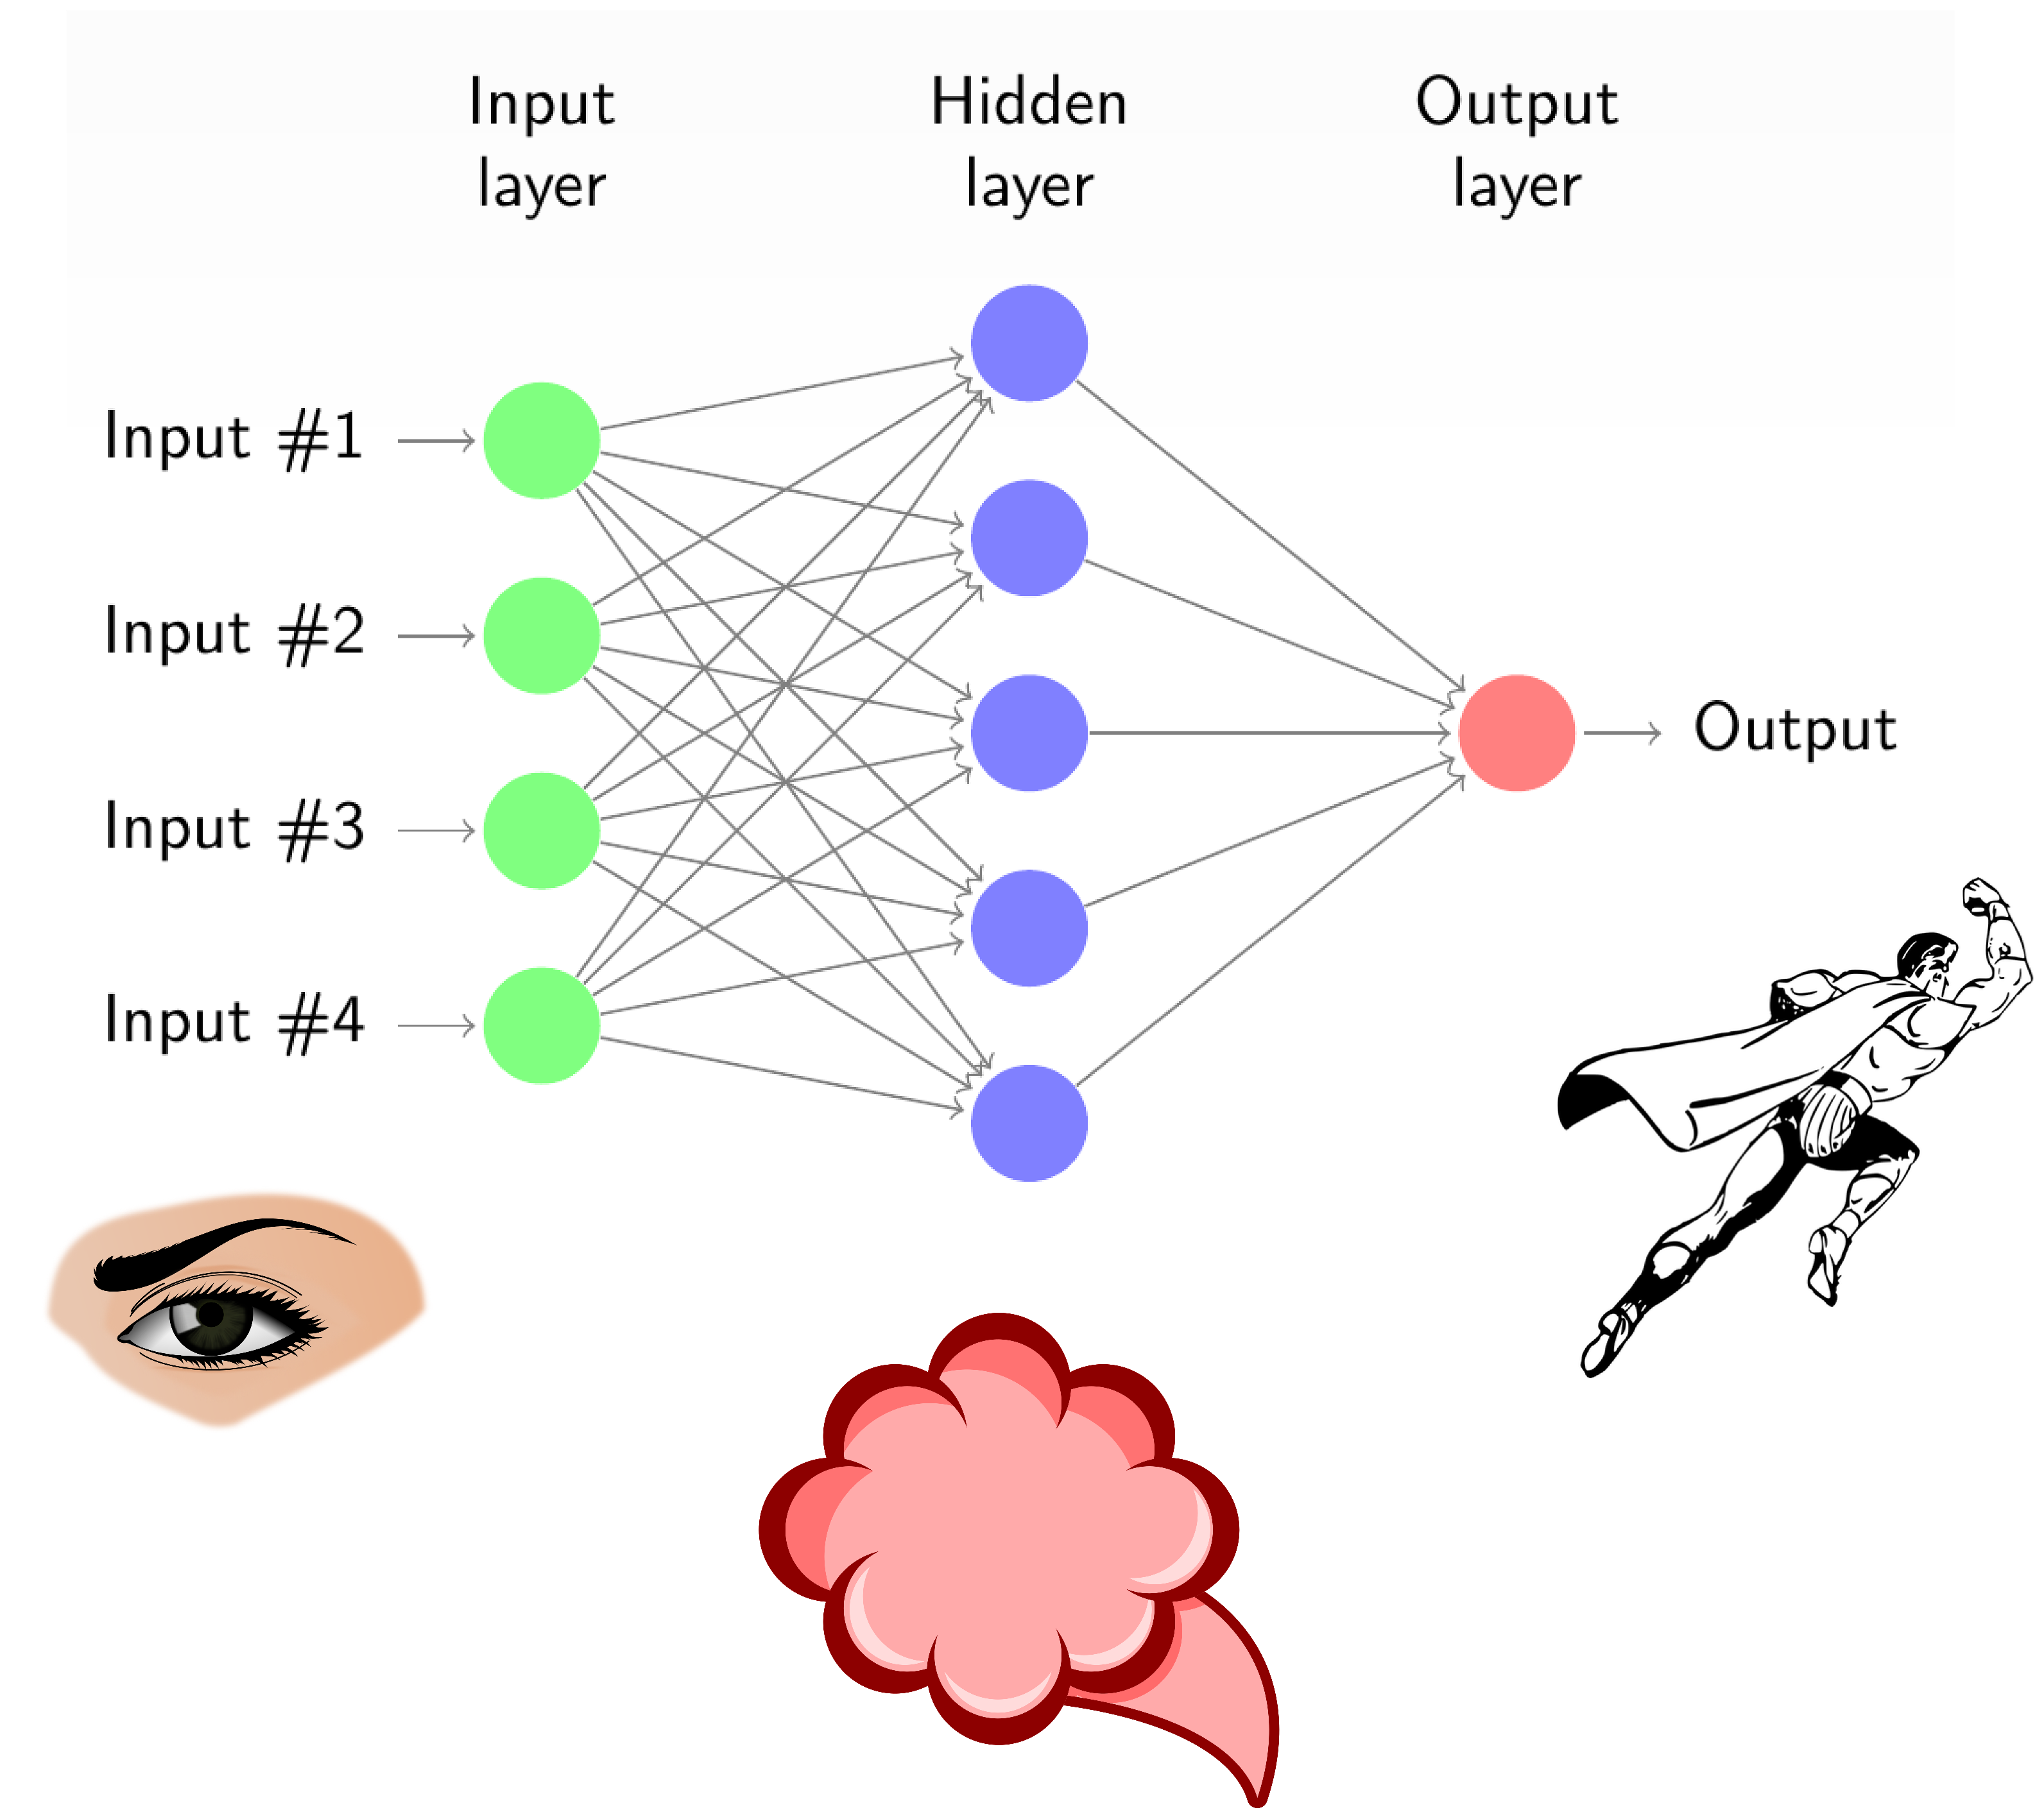
\includegraphics[width=0.8\textwidth]{net_structure}
\end{figure}
\end{frame}

\begin{frame}{Neural Networks - Processing information}
\begin{tabular}{p{5cm}|p{5cm}}
    \begin{figure}
    	
\includegraphics[scale = 0.09]{brain}
    \end{figure}
    & 
    \begin{figure}
    	
\includegraphics[scale = 1.4]{machine}
    \end{figure} \\
  \multicolumn{1}{c|}{Evaluation of an action} & \multicolumn{1}{c}{Loss function} \\
    \begin{itemize}
        \item Simple perceptions: pain, satisfaction
        \item Expectation
    \end{itemize}
    & 
    \begin{itemize}
      \item Supervised learning: compare to the desired outcome
      \item Loss = estimator for quality
    \end{itemize} \\
\multicolumn{1}{c|}{Decision for a next step} & \multicolumn{1}{c}{Optimisation} \\
    \begin{itemize}
        \item Trial and error
        \item Learning from experience
    \end{itemize}
    & 
    \begin{itemize}
      \item Back-propagation impact of parameters' on the loss
      \item Adjust parameters to minimise plot
    \end{itemize} 
 \end{tabular}
\end{frame}



